\section{System Model and Problem Formulation}
\label{sec:system_model}

\subsection{Edge-Cloud IoT Architecture}

The system contains IoT devices, edge nodes, cloud nodes, and a scheduling broker. Devices generate tasks over discrete timesteps. Each task is associated with one nearby edge node, but the scheduler can choose either edge execution or cloud execution. Edge execution uses local compute and memory near the device. Cloud execution uses remote capacity and includes uplink, network, queue, and cloud processing delay.

\begin{figure*}[!t]
\centering
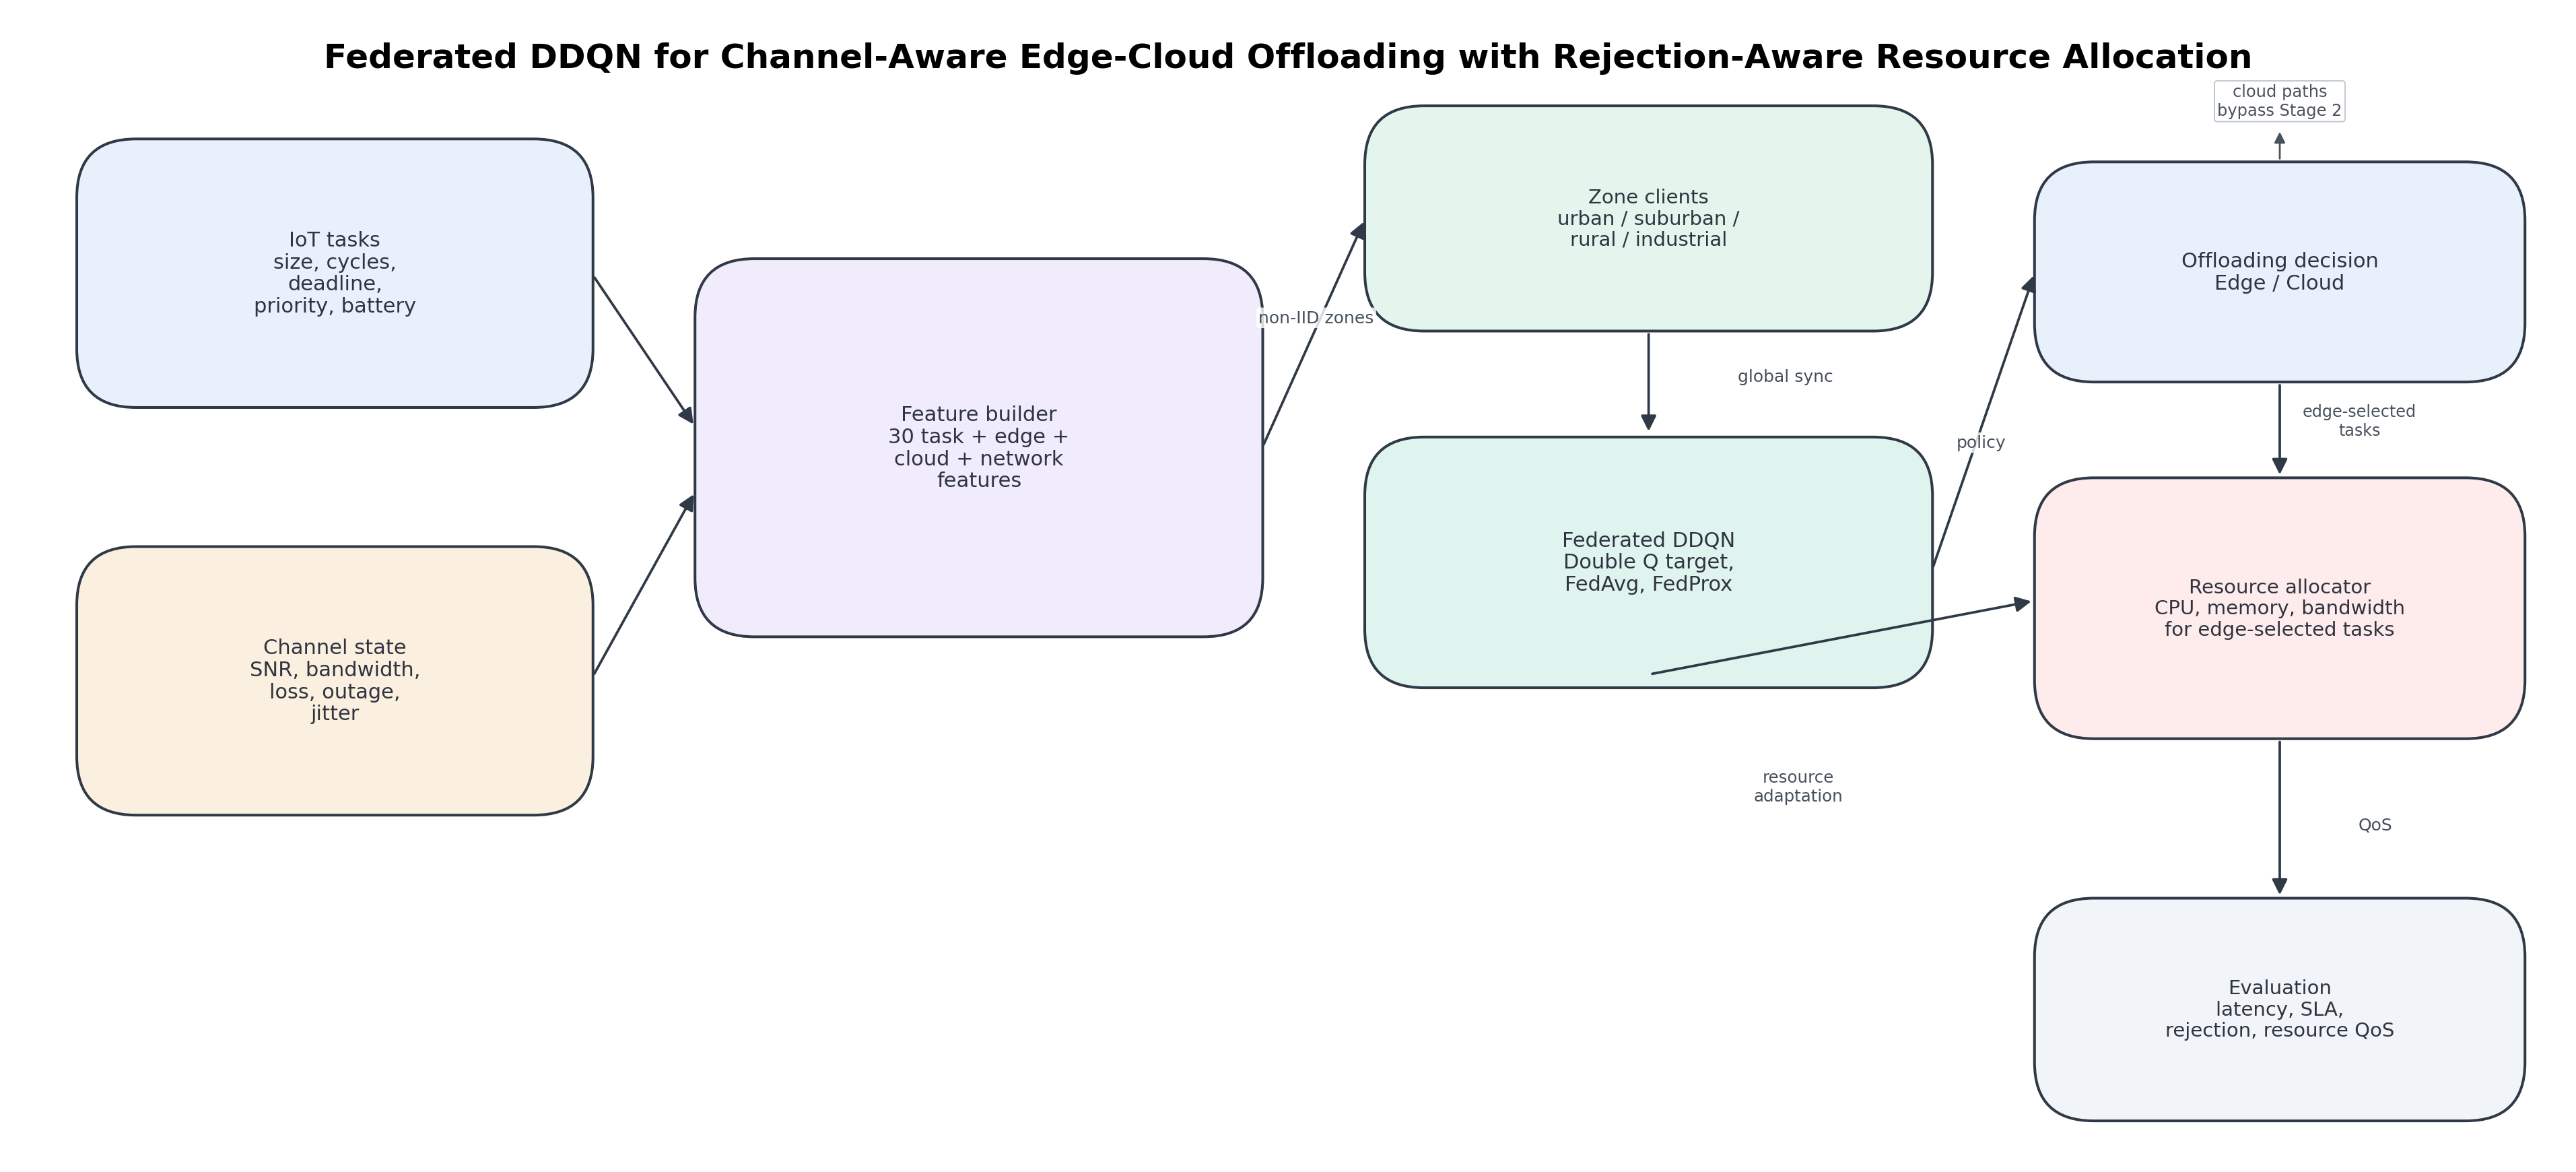
\includegraphics[width=0.84\textwidth]{figures/diagrams/150_fig_a1_system_architecture.png}
\caption{Two-stage edge-cloud IoT system. Stage 1 is the proposed federated DDQN offloading policy. Stage 2 applies rejection-aware resource allocation only to tasks selected for edge execution.}
\label{fig:architecture}
\end{figure*}

Let $\mathcal{E}=\{1,\ldots,E\}$ denote the set of edge nodes and $\mathcal{C}=\{1,\ldots,C\}$ denote the set of cloud nodes. In \dataset{}, $E=50$ and $C=10$. Let $t\in\{1,\ldots,T\}$ be the timestep, with $T=1000$. Edge node $j$ at time $t$ has CPU availability $u^e_{j,t}$, memory availability $m^e_{j,t}$, queue length $q^e_{j,t}$, energy state $\eta^e_{j,t}$, and fault state $f^e_{j,t}$. The network state at time $t$ is $n_t$, which includes uplink bandwidth, downlink bandwidth, packet loss, signal-to-noise ratio (SNR), base delay, outage state, congestion state, and jitter state. Cloud node $k$ has CPU availability $u^c_{k,t}$, memory availability $m^c_{k,t}$, queue length $q^c_{k,t}$, and maintenance or overload indicators.

\begin{table*}[!t]
\centering
\caption{Main notation for the edge-cloud offloading problem.}
\label{tab:problem_notation}
\scriptsize
\begin{tabularx}{\textwidth}{@{}lX@{}}
\toprule
Symbol & Meaning \\
\midrule
$\tau_i$ & Task $i$ with size, compute, memory, deadline, priority, security, battery, type, arrival time, and assigned edge node. \\
$\kappa_i$ & Task type/category, such as emergency, video, AI, telemetry, or firmware update. \\
$t_i$ & Arrival timestep of task $i$. \\
$j_i$ & Edge node associated with task $i$ by locality. \\
$a_i$ & Binary offloading action, where $0$ denotes edge execution and $1$ denotes cloud execution. \\
$x_i$ & Engineered feature vector used by the Stage-1 policy. \\
$L_i^e$, $L_i^c$ & Estimated edge and cloud latency for task $i$. \\
$L_i(a_i)$, $\tilde{L}_i(a_i)$ & Selected latency and normalized selected latency under action $a_i$. \\
$L_i^{\mathrm{best}}$, $L_i^{\mathrm{worst}}$ & Minimum and maximum finite generated latency over edge/cloud alternatives after infeasible sentinel values are excluded for reward shaping. \\
$\delta_i$ & Task-specific deadline or SLA threshold. \\
$M_i$ & SLA-miss indicator, equal to $1-\mathrm{SLA}_i$. \\
$\Phi_i^e$, $\Phi_i^c$, $\Phi_i(a_i)$ & Edge, cloud, and selected-path feasibility predicates used to compute selected-path rejection. \\
$F_i$ & Selected-path feasibility or admission failure indicator. \\
$R_i$ & Reported rejection indicator, equal to selected-path feasibility or admission failure $F_i$. \\
$Q_i$ & Broad QoS-failure indicator, $Q_i=\mathbb{I}[M_i=1\lor F_i=1]$, used only when a union of SLA miss and rejection is needed. \\
$\hat{\rho}_i$ & Pre-decision QoS/admission-risk estimate from observable task, channel, queue, and feasibility predictors; distinct from realized outcomes $M_i$, $R_i$, and $Q_i$. \\
$u_i^{\min}$, $\bar{m}_i$ & Normalized CPU and memory feasibility thresholds for task $i$ in the generated resource-availability scale. \\
$u^e_{j,t}$, $m^e_{j,t}$ & Edge CPU and memory availability for node $j$ at time $t$. \\
$q^e_{j,t}$ & Edge queue length for node $j$ at time $t$. \\
$n_t$ & Network state at time $t$, including bandwidth, delay, packet loss, SNR, outage, congestion, and jitter indicators. \\
$\theta$, $\theta^-$ & Online and target Q-network parameters. \\
$\theta_z$, $\theta_g$ & Local zone model and current global federated model. \\
$\mathbf{y}_i^{*}$ & Generated Stage-2 proxy target for CPU, memory, and bandwidth allocation on allocator-valid edge-selected tasks. \\
$\hat{\mathbf{y}}_i$ & Stage-2 predicted/final CPU, memory, and bandwidth allocation for edge-selected task $i$. \\
$\mathcal{G}^{\mathrm{valid}}_e(j,t)$ & Allocator-valid edge-selected tasks sharing edge node $j$ and timestep $t$ for Stage-2 group-wise capacity normalization. \\
\bottomrule
\end{tabularx}
\end{table*}

\begin{table*}[!t]
\centering
\caption{Additional method notation and implementation parameters.}
\label{tab:method_parameters}
\scriptsize
\begin{tabularx}{\textwidth}{@{}lX@{}}
\toprule
Symbol & Meaning in this benchmark implementation \\
\midrule
$u_i^{\min}$ & Minimum normalized edge CPU availability required by task $i$ after converting demand to the generator-native availability scale. \\
$\bar{m}_i$ & Minimum normalized edge memory availability required by task $i$ after converting memory demand to the generator-native availability scale. \\
$P_i^e$ & Edge-pressure penalty used when local queue, edge overload, or edge-overuse risk makes an edge decision less desirable. \\
$H_i$ & Heavy-task edge-misrouting indicator for AI, video, image, and firmware-like tasks when cloud execution is predicted to be safer or faster. \\
$h_i$ & Compact heavy-task flag used in margin and allocator formulas; $h_i=1$ for cloud-favorable heavy task categories and $0$ otherwise. \\
$\bar{\delta}_i$ & Deadline-tightness score for task $i$; larger values mean tighter deadlines after normalization. \\
$\chi_i^{\mathrm{rt}}$ & Binary real-time task flag used in Stage-2 urgency and allocation-target generation. \\
$\mathcal{G}^{\mathrm{valid}}_e(j,t)$ & Allocator-valid edge-selected task group sharing edge node $j$ and timestep $t$ in the Stage-2 normalization pass. \\
$C^r_{j,t}$ & Normalized available capacity of edge node $j$ for resource channel $r\in\{\mathrm{cpu},\mathrm{mem},\mathrm{bw}\}$ at time $t$. \\
$\epsilon$ & Small positive constant used in denominators and projection formulas to avoid division by zero. \\
$\alpha_{\mathrm{res}},\alpha_{\mathrm{dem}}$ & Fixed blend weights for the Stage-2 residual and rejection-aware demand branches; the implementation uses $0.10$ and $0.90$, respectively. \\
$\omega_i$ & Bounded Stage-2 demand multiplier derived from urgency and pre-decision QoS/admission-risk features. \\
$\rho_i^{\mathrm{sla}}$ & Pre-decision edge-SLA-risk component used inside the Stage-2 rejection-aware demand branch. \\
$\mathbf{d}^{\mathrm{raw}}_i$ & Bounded demand-score vector used before Stage-2 demand-branch capacity normalization. \\
$z_i$ & Allocator input vector containing task, state, policy-output, demand, and pre-decision risk features for task $i$. \\
$f_{\phi}$ & Residual resource-allocation network parameterized by $\phi$. \\
$\zeta_i^{\mathrm{term}}$ & Binary terminal-mask indicator for the DDQN target; it is one at split, gap, sequence, or final-sample boundaries where bootstrapping is suppressed. \\
\bottomrule
\end{tabularx}
\end{table*}


\subsection{Task Model}

A task $i$ arriving at time $t_i$ is represented by $\tau_i=(d_i,c_i,m_i,\delta_i,p_i,\allowbreak s_i,b_i,\kappa_i,t_i,j_i)$, where $d_i$ is input size, $c_i$ is CPU demand, $m_i$ is memory demand, $\delta_i$ is the deadline, $p_i$ is priority, $s_i$ captures security sensitivity, $b_i$ captures battery state, $\kappa_i$ is task type, and $j_i$ is the assigned edge node. Task type matters because emergency, video, telemetry, and firmware tasks can have different urgency and compute patterns even at similar sizes.

The task and state columns are generator-native quantities rather than direct measurements from one physical deployment. Size, demand, bandwidth, and availability are converted into normalized pressure or availability features before learning. Formulas such as $c_i/u^e_{j,t}$ and $d_i/B^{\mathrm{eff}}_t$ are therefore benchmark-consistent service-pressure terms, not calibrated processor or radio measurements.

The scheduler chooses a binary action $a_i\in\{0,1\}$, where $0$ denotes edge execution and $1$ denotes cloud execution. The binary action space keeps the decision interpretable. Rejection is not an action. It is an outcome that can occur after the selected destination is checked against resource, security, and deadline feasibility.

\subsection{Edge Execution Model}

If $a_i=0$, task $i$ is executed at edge node $j_i$. Its edge latency is modeled as
\begin{equation}
L_i^{e} = L^{e,\mathrm{queue}}_{i} + L^{e,\mathrm{exec}}_{i} + L^{e,\mathrm{local}}_{i} + L^{e,\mathrm{fault}}_{i},
\label{eq:edge_latency}
\end{equation}
where $L^{e,\mathrm{queue}}_i$ increases with $q^e_{j_i,t_i}$ and recent arrivals, $L^{e,\mathrm{exec}}_i$ depends on $c_i/u^e_{j_i,t_i}$, $L^{e,\mathrm{local}}_i$ represents local transfer and broker overhead, and $L^{e,\mathrm{fault}}_i$ captures degradation, isolation, or failure penalties. Edge execution is feasible only when generated resource, node-state, security, battery, corruption, and admission checks pass:
\begin{equation}
\begin{aligned}
\Phi_i^e={}&
\Phi_{i,\mathrm{cpu}}^e
\land \Phi_{i,\mathrm{mem}}^e
\land \Phi_{i,\mathrm{state}}^e
\land \Phi_{i,\mathrm{sec}}^e \\
&\land \Phi_{i,\mathrm{bat}}^e
\land \Phi_{i,\mathrm{corr}}^e
\land \Phi_{i,\mathrm{adm}}^e .
\end{aligned}
\label{eq:edge_feasibility}
\end{equation}
Here $\Phi_{i,\mathrm{cpu}}^e$ includes $u^e_{j_i,t_i}\geq u_i^{\min}$, $\Phi_{i,\mathrm{mem}}^e$ includes $m^e_{j_i,t_i}\geq \bar{m}_i$, and $\Phi_{i,\mathrm{state}}^e$ excludes failed or isolated edge states. The remaining terms encode security compatibility, battery or local-device restrictions, corrupt-task flags, and generator-side deadline/admission consistency. The implementation uses lookup tables from the generated CSV state files rather than recomputing each term from a closed-form physical model. Equations~\eqref{eq:edge_latency} and \eqref{eq:edge_feasibility} describe the conceptual decomposition used to interpret those computed labels.

\subsection{Cloud Execution Model}

If $a_i=1$, the task is sent to the cloud. Its latency is
\begin{equation}
L_i^{c}=L^{\mathrm{up}}_i + L^{n}_t + L^{c,\mathrm{queue}}_i + L^{c,\mathrm{exec}}_i + L^{c,\mathrm{cold}}_i,
\label{eq:cloud_latency}
\end{equation}
where $L^{\mathrm{up}}_i$ depends on task size and uplink bandwidth, $L^n_t$ is network delay, $L^{c,\mathrm{queue}}_i$ is cloud queue delay, $L^{c,\mathrm{exec}}_i$ is cloud processing delay, and $L^{c,\mathrm{cold}}_i$ accounts for cold starts, overload, and maintenance windows. Cloud execution can be attractive for large compute tasks when edge resources are scarce. It is less attractive when the network state is degraded or when the deadline is tight. Cloud feasibility is written analogously:
\begin{equation}
\begin{aligned}
\Phi_i^c={}&
\Phi_{i,\mathrm{cpu}}^c
\land \Phi_{i,\mathrm{mem}}^c
\land \Phi_{i,\mathrm{state}}^c
\land \Phi_{i,\mathrm{net}}^c \\
&\land \Phi_{i,\mathrm{sec}}^c
\land \Phi_{i,\mathrm{corr}}^c
\land \Phi_{i,\mathrm{adm}}^c .
\end{aligned}
\label{eq:cloud_feasibility}
\end{equation}
The cloud resource terms cover generated cloud CPU and memory availability, $\Phi_{i,\mathrm{state}}^c$ covers maintenance, overload, and cold-start state, and $\Phi_{i,\mathrm{net}}^c$ covers outage, packet-loss, and effective-bandwidth admission. Security, corrupt-task, and deadline/admission consistency are checked on the selected cloud path in the same way they are checked on the selected edge path.

\subsection{QoS and Rejection Outcomes}

A task satisfies its SLA if the selected latency is no greater than the task-specific deadline:
\begin{equation}
\mathrm{SLA}_i = \mathbb{I}\left[L_i(a_i) \leq \delta_i\right],
\label{eq:sla_flag}
\end{equation}
where $L_i(a_i)=L_i^e$ for edge execution and $L_i(a_i)=L_i^c$ for cloud execution. The SLA-miss indicator is
\begin{equation}
M_i=1-\mathrm{SLA}_i.
\label{eq:sla_miss}
\end{equation}
The selected path may also fail feasibility or admission checks. The selected-path predicate is
\begin{equation}
\Phi_i(a_i)=
\begin{cases}
\Phi_i^e, & a_i=0,\\
\Phi_i^c, & a_i=1.
\end{cases}
\label{eq:selected_feasibility}
\end{equation}
The failure indicator and reported rejection metric are then
\begin{align}
F_i &= \mathbb{I}\left[\neg \Phi_i(a_i)\right], \\
R_i &= F_i.
\label{eq:rejection_flag}
\end{align}
Thus $R_i$ is not a third scheduler action and is not the same as an SLA miss. It is the feasibility or admission failure of the path that the policy selected.
For discussion that needs a broader QoS-failure indicator, define
\begin{equation}
Q_i=\mathbb{I}\left[M_i=1 \;\lor\; F_i=1\right].
\label{eq:qos_failure_flag}
\end{equation}
Thus, SLA miss, rejection, and broad QoS failure are related but not identical. $M_i$ records latency-deadline violation, $R_i$ records selected-path infeasibility or admission failure, and $Q_i$ records their union. The policy is not rewarded for choosing rejection because rejection is not an action; it is an outcome of the selected edge or cloud path.

The pre-decision QoS/admission-risk estimate is denoted by $\hat{\rho}_i$. It is different from the realized outcomes $M_i$, $R_i$, and $Q_i$: $\hat{\rho}_i$ is computed before action evaluation from observable risk predictors such as deadline tightness, low battery, corruption flags, local queue pressure, outage/congestion state, and destination availability. It is used for reward shaping and Stage-2 allocation, while $M_i$ and $R_i$ are computed only after the selected edge or cloud path is evaluated. Aggregate latency is computed on valid held-out rows from the selected edge/cloud latency table; SLA miss and rejection are then computed from the selected path and benchmark feasibility flags.

\subsection{Latency-Reference Oracle}

The Oracle reported in the results is a non-trainable latency reference over the generated edge and cloud alternatives. Let $L_{\mathrm{sent}}$ denote the sentinel value used by the label-generation pipeline for invalid or unavailable latency entries. The Oracle action is
\begin{equation}
a_i^{\mathrm{orc}} =
\arg\min_{a\in\{0,1\}: L_i(a)<L_{\mathrm{sent}}} L_i(a),
\qquad
L_i^{\mathrm{orc}}=L_i(a_i^{\mathrm{orc}}).
\label{eq:oracle_rule}
\end{equation}
This rule bounds the generated latency achievable by a binary edge/cloud decision on the offline sequence. It is not a deployable policy, and it is not a universal ceiling for every QoS metric. Oracle SLA miss and rejection can remain nonzero because the rule minimizes finite generated latency among available alternatives; it does not guarantee that every task is feasible or deadline-satisfying.

\subsection{Problem Objective}

The offloading objective is to find a policy $\pi(a|x_i)$ that minimizes expected latency and QoS penalties:
\begin{equation}
\begin{aligned}
\min_{\pi}\quad &\mathbb{E}_{i}\big[
\tilde{L}_i(a_i)
+\lambda_{\mathrm{sla}}M_i
+\lambda_{\mathrm{rej}}R_i \\
&\quad
+\lambda_{\mathrm{edge}}P^e_i
+\lambda_{\mathrm{heavy}}H_i
\big],
\end{aligned}
\label{eq:objective}
\end{equation}
subject to edge, cloud, and network feasibility constraints. Here $x_i$ is the 30-dimensional feature vector, $\tilde{L}_i(a_i)$ is normalized selected latency, $P^e_i$ is an edge-pressure penalty, and $H_i$ penalizes routing heavy cloud-favorable tasks to edge when that choice is predicted to be harmful. The $\lambda$ terms control the relative cost of SLA miss, selected-path rejection, overload, and heavy-task mismatch.

If raw latency is used in an implementation, the corresponding $\lambda$ values are interpreted in latency-equivalent units. The proposed \fedddqn{} learns this decision rule through offline replay over the fixed benchmark sequence: policy actions determine the reward for the sampled task, but the next task/state is exogenous and precomputed instead of being mutated online by the selected action. The final test evaluation then applies the learned policy to a held-out temporal interval.
